\documentclass[border=8pt]{standalone}
\usepackage{amsmath}
\usepackage{pgfplots}
\pgfplotsset{compat=1.18}
\begin{document}
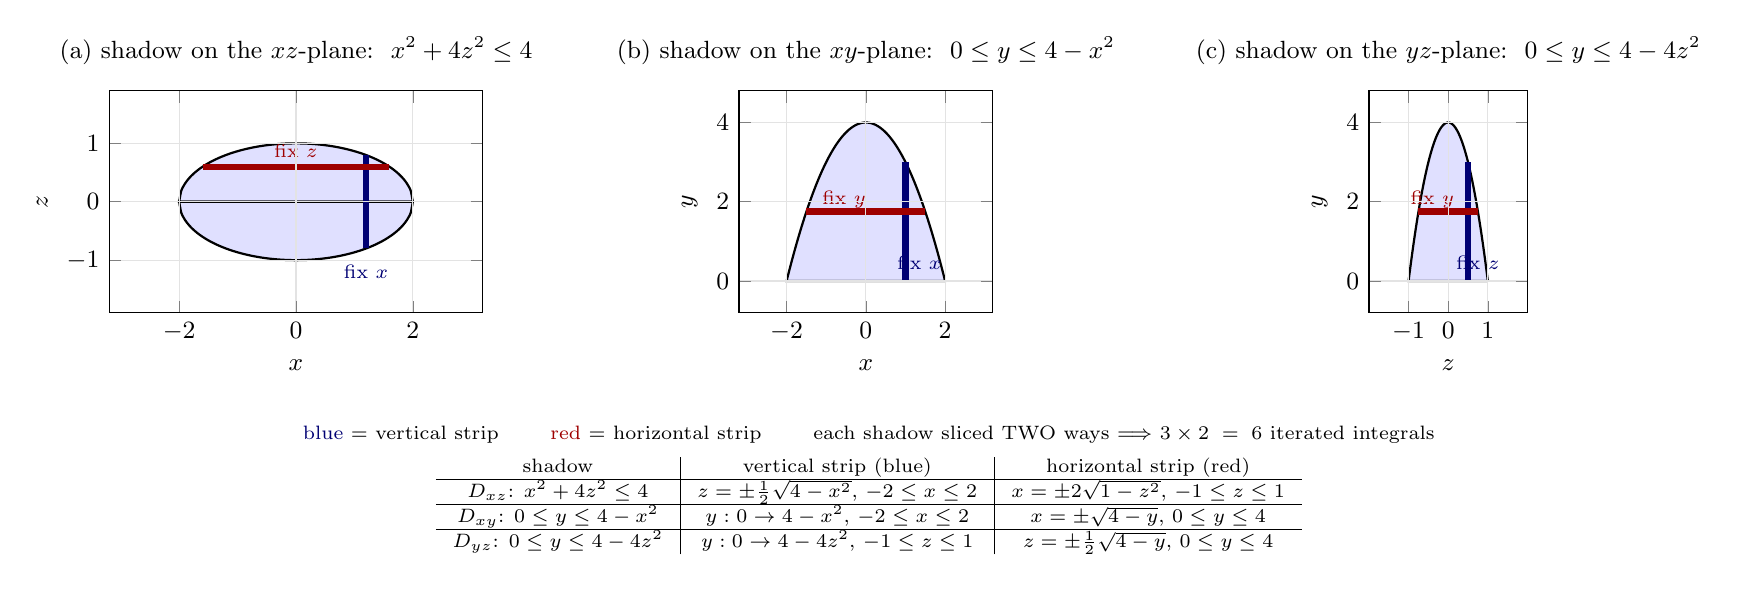
\begin{tikzpicture}[font=\small,
  bluestrip/.style={blue!45!black, line width=2.3pt},
  redstrip/.style ={red!62!black, line width=2.3pt}]

% ===================== (a) shadow on the xz-plane ==========================
\begin{axis}[
    width=6.4cm, height=4.4cm, axis equal image,
    xlabel=$x$, ylabel=$z$,
    title={(a)  shadow on the $xz$-plane:\ \ $x^2+4z^2\le 4$},
    xmin=-3.2, xmax=3.2, ymin=-1.9, ymax=1.9,
    xtick={-2,0,2}, ytick={-1,0,1},
    grid=major, grid style={gray!22, line width=.4pt}, axis on top]
  \addplot[fill=blue!12, draw=black, thick, domain=-2:2, samples=121, smooth]
      ({x},{sqrt(4-x^2)/2}) \closedcycle;
  \addplot[fill=blue!12, draw=black, thick, domain=-2:2, samples=121, smooth]
      ({x},{-sqrt(4-x^2)/2}) \closedcycle;
  \addplot[bluestrip, forget plot] coordinates {(1.2,-0.8) (1.2,0.8)};
  \addplot[redstrip,  forget plot] coordinates {(-1.6,0.6) (1.6,0.6)};
  \node[font=\scriptsize, blue!45!black] at (axis cs:1.2,-1.2) {fix $x$};
  \node[font=\scriptsize, red!62!black]  at (axis cs:0,0.88) {fix $z$};
\end{axis}

% ===================== (b) shadow on the xy-plane ==========================
\begin{scope}[xshift=8.0cm]
\begin{axis}[
    width=6.4cm, height=4.4cm, axis equal image,
    xlabel=$x$, ylabel=$y$,
    title={(b)  shadow on the $xy$-plane:\ \ $0\le y\le 4-x^2$},
    xmin=-3.2, xmax=3.2, ymin=-0.8, ymax=4.8,
    xtick={-2,0,2}, ytick={0,2,4},
    grid=major, grid style={gray!22, line width=.4pt}, axis on top]
  \addplot[fill=blue!12, draw=black, thick, domain=-2:2, samples=121, smooth]
      ({x},{4-x^2}) \closedcycle;
  \addplot[bluestrip, forget plot] coordinates {(1,0) (1,3)};
  \addplot[redstrip,  forget plot] coordinates {(-1.5,1.75) (1.5,1.75)};
  \node[font=\scriptsize, blue!45!black] at (axis cs:1.35,0.45) {fix $x$};
  \node[font=\scriptsize, red!62!black]  at (axis cs:-0.55,2.05) {fix $y$};
\end{axis}
\end{scope}

% ===================== (c) shadow on the yz-plane ==========================
\begin{scope}[xshift=16.0cm]
\begin{axis}[
    width=6.4cm, height=4.4cm, axis equal image,
    xlabel=$z$, ylabel=$y$,
    title={(c)  shadow on the $yz$-plane:\ \ $0\le y\le 4-4z^2$},
    xmin=-2.0, xmax=2.0, ymin=-0.8, ymax=4.8,
    xtick={-1,0,1}, ytick={0,2,4},
    grid=major, grid style={gray!22, line width=.4pt}, axis on top]
  \addplot[fill=blue!12, draw=black, thick, domain=-1:1, samples=121, smooth]
      ({x},{4-4*x^2}) \closedcycle;
  \addplot[bluestrip, forget plot] coordinates {(0.5,0) (0.5,3)};
  \addplot[redstrip,  forget plot] coordinates {(-0.75,1.75) (0.75,1.75)};
  \node[font=\scriptsize, blue!45!black] at (axis cs:0.75,0.45) {fix $z$};
  \node[font=\scriptsize, red!62!black]  at (axis cs:-0.4,2.05) {fix $y$};
\end{axis}
\end{scope}

% ===================== summary table underneath ============================
\node[font=\scriptsize, align=center, yshift=-1.4cm] at (current bounding box.south)
  {\textcolor{blue!45!black}{blue} $=$ vertical strip \qquad
   \textcolor{red!62!black}{red} $=$ horizontal strip \qquad
   each shadow sliced TWO ways $\Longrightarrow$ $3\times 2\;=\;6$ iterated integrals\\[4pt]
   \begin{tabular}{c|c|c}
     shadow & vertical strip (blue) & horizontal strip (red)\\\hline
     $D_{xz}$: $x^2+4z^2\le 4$   & $z=\pm\tfrac{1}{2}\sqrt{4-x^2}$,\ $-2\le x\le 2$
                                  & $x=\pm 2\sqrt{1-z^2}$,\ $-1\le z\le 1$\\\hline
     $D_{xy}$: $0\le y\le 4-x^2$ & $y:0\to 4-x^2$,\ $-2\le x\le 2$
                                  & $x=\pm\sqrt{4-y}$,\ $0\le y\le 4$\\\hline
     $D_{yz}$: $0\le y\le 4-4z^2$& $y:0\to 4-4z^2$,\ $-1\le z\le 1$
                                  & $z=\pm\tfrac{1}{2}\sqrt{4-y}$,\ $0\le y\le 4$\\
   \end{tabular}};
\end{tikzpicture}
\end{document}
